\documentclass[a4paper, 14pt]{extarticle}
\usepackage[russian]{babel}
\usepackage[T1]{fontenc}
\usepackage{fontspec}
\usepackage{indentfirst}
\usepackage{enumitem}
\usepackage{graphicx}
\usepackage{scrextend}
\usepackage{longtable}
\usepackage[
  left=20mm,
  right=10mm,
  top=20mm,
  bottom=20mm
]{geometry}
\usepackage{parskip}
\usepackage{titlesec}
\usepackage{xurl}
\usepackage{hyperref}
\usepackage{float}
\usepackage[
  figurename=Рисунок,
  labelsep=endash,
]{caption}
\usepackage[outputdir=build, newfloat]{minted}
\usepackage{multirow}
\usepackage{array}

\hypersetup{
  colorlinks=true,
  linkcolor=black,
  filecolor=blue,
  urlcolor=blue,
}

\renewcommand*{\labelitemi}{---}
\setmainfont{Times New Roman}
\setmonofont{JetBrains Mono}[
  SizeFeatures={Size=11},
]

\newenvironment{code}{\captionsetup{type=listing}}{}
\SetupFloatingEnvironment{listing}{name=Листинг}

\setminted{
  fontsize=\footnotesize,
  framesep=0mm,
}

\captionsetup{width=\textwidth,justification=centering}
\captionsetup[table]{singlelinecheck=off,justification=justified}

\newcolumntype{L}[1]{>{\raggedright\let\newline\\\arraybackslash\hspace{0pt}}m{#1}}
\newcolumntype{C}[1]{>{\centering\let\newline\\\arraybackslash\hspace{0pt}}m{#1}}
\newcolumntype{R}[1]{>{\raggedleft\let\newline\\\arraybackslash\hspace{0pt}}m{#1}}

\setlength{\parskip}{6pt}

\setlength{\parindent}{1cm}
\setlist[itemize]{itemsep=0em,topsep=0em,parsep=0em,partopsep=0em,leftmargin=2.0cm}
\setlist[enumerate]{itemsep=0em,topsep=0em,parsep=0em,partopsep=0em,leftmargin=2.0cm}

\renewcommand{\thesection}{\arabic{section}.}
\renewcommand{\thesubsection}{\thesection\arabic{subsection}.}
\renewcommand{\thesubsubsection}{\thesubsection\arabic{subsubsection}.}

\titleformat{\section}{\normalfont\bfseries}{\thesection}{0.5em}{}
\titleformat{\subsection}{\normalfont\bfseries}{\thesubsection}{0.5em}{}

\titleformat*{\section}{\normalfont\bfseries}
\titleformat*{\subsection}{\normalfont\bfseries}

\linespread{1.5}
\renewcommand{\baselinestretch}{1.5}

\renewcommand{\theenumii}{(\asbuk{enumii})}
\renewcommand{\labelenumii}{\asbuk{enumii})}
\AddEnumerateCounter{\asbuk}{\@asbuk}{\cyrm}

\begin{document}

\begin{titlepage}
  \vspace{0pt plus2fill}
  \noindent

  \vspace{0pt plus6fill}
  \begin{center}
    Санкт-Петербургский национальный исследовательский университет
    информационных технологий, механики и оптики

    \vspace{0pt plus2fill}

    Практическая работа по теме:

    <<Разработка спецификации требований к программному обеспечению>>

    \vspace{0pt plus1fill}

    Задание №7

    <<Реализация диаграммы взаимодействия>>

  \end{center}

  \vspace{0pt plus7fill}
  \begin{flushright}
    Выполнил: \\
    Швалов Даниил Андреевич

    Группа: К33211

    Проверил: \\
    Осипов Никита Алексеевич
  \end{flushright}

  \vspace{0pt plus2fill}
  \begin{center}
    Санкт-Петербург

    2023
  \end{center}
\end{titlepage}

\setcounter{page}{2}

\section{Введение}

\textbf{Цель работы}: освоить методику проектирования реализации прецедентов,
изучить шаблоны GRASP для распределения обязанностей между классами.

\section{Ход работы}

\subsection{Шаблоны GRASP}

\subsubsection*{Creator}

Шаблон Creator используется для определения класса, ответственного за создание
других классов. Класс, которого планируется наделить ответственностью создателя,
должен отвечать одному или нескольким из следующих требований:
\begin{itemize}
  \item создатель содержит или агрегирует объекты, которые необходимо создавать;
  \item создатель записывает экземпляры объектов, которые необходимо создавать;
  \item создатель активно использует объекты, которые необходимо создавать;
  \item создатель обладает данными инициализации для объектов, которые
  необходимо создавать.
\end{itemize}
В ЕГСА шаблон Creator применим к системе подаче документов. При подаче
документов абитуриент заполняет все сведения о себе, после чего система создает
заявление на поступление. Другими словами, класс <<Системы заявлений>> создает
класс <<Заявление на поступление>>.

\subsubsection*{Information Expert}

Шаблон Information Expert используется для определения класса, ответственного за
предоставление информации о конкретном объекте. Для определения класса, который
будет ответственным за предоставление информации о конкретном объекте,
необходимо выяснить, какой класс обладает достаточной информацией для этого. В
случае ЕГСА шаблон Information Expert может быть применим для отслеживания
статуса заявления. Абитуриент, который хочет узнать статус своего заявления,
должен обратиться к системе заявлений. Другими словами, класс <<Системы
заявлений>> содержит информацию о классе <<Заявление на поступление>>.

\subsubsection*{Low Coupling}

Шаблон Low Coupling используется для оценки существующего проектного решения или
выбора решения из нескольких вариантов. При прочих равных условиях следует
предпочитать проектное решение с более низкой степенью связывания. Так,
например, в ЕГСА класс <<Абитуриент>> не должен хранить в себе информацию о
своих заявлениях, они должны храниться только в <<Системе заявлений>>. Такой
подход позволит снизить связность и повысить гибкость и расширяемость системы.

\subsubsection*{Controller}

Шаблон Controller используется для определения класса, который должен отвечать
за обработку запросов и решать кому должен делегировать запросы на выполнение.
Класс, которому планируется присвоить эту обязанность, должен удовлетворять
одним из следующих условий:
\begin{itemize}
  \item класс представляет всю систему в целом, корневой объект, устройство или
  важную подсистему;
  \item класс представляет сценарий некоторого прецедента, в рамках которого
  выполняется обработка этой системной операции.
\end{itemize}
В ЕГСА шаблон Controller применим, например, к общей системе, к которой
обращается пользователь, которая, в свою очередь, вызывает остальные подсистемы
для выполнения той или иной операции. Другими словами, класс <<Система
абитуриента>> делегирует запрос классу <<Система заявлений>> при создании
заявления на поступлении.

\subsubsection*{High Cohesion}

Шаблон High Cohesion используется для обеспечения сфокусированности обязанностей
объектов, улучшения их управляемости и ясности засчет распределения
обязанностей. Этот шаблон нужно использовать для оценки вариантов при выборе
решения. В ЕГСА, например, <<Система абитуриента>> не должна выполнять всю
функциональность, которую она предоставляет. Большая ее часть должна быть
вынесена в подсистемы.

\subsection{Диаграмма взаимодействия}

На рис. \ref{fig:diagram} приведен пример диаграммы взаимодействия, на которой
изображен процесс работы системы при подаче заявления на поступление
абитуриентом.

\begin{figure}[H]
  \centering
  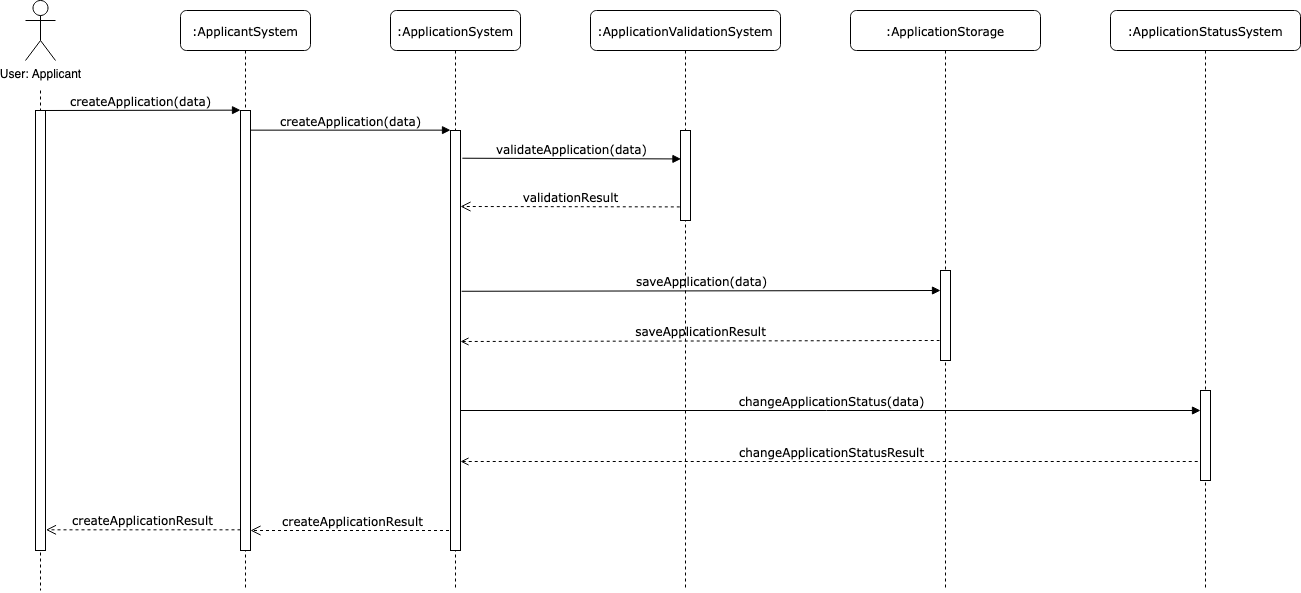
\includegraphics[width=\textwidth]{images/diagram.png}
  \caption{Пример диаграммы взаимодействия}
  \label{fig:diagram}
\end{figure}

\newpage

\section{Заключение}

В ходе выполнения практического задания была освоена методика проектирования
реализации прецедентов и изучены шаблоны GRASP для распределения обязанностей
между классами.

\end{document}
